\documentclass[12pt,a4paper]{scrartcl}
\usepackage[utf8]{inputenc}
\usepackage[T1]{fontenc}
\usepackage{ngerman}
\usepackage{placeins}
%\usepackage[ngerman]{babel}  % use babel for multi-ling or english
%
%\usepackage{amsmath,amssymb,amstext}

\usepackage{amsmath}
\usepackage{wrapfig}
\usepackage{multirow}
%\usepackage{sv}
\usepackage{pgf}
\usepackage{pst-sigsys}
\usepackage{multido}
\usepackage{pdfpages}
\usepackage{listings}
\usepackage{color}
\definecolor{light-gray}{gray}{0.95}


% fuer Zitate
\usepackage[numbers]{natbib}
\usepackage{nomencl,longtable} 
% Festlegung Art der Zitierung - Havardmethode: Abkuerzung Autor + Jahr
%\bibliographystyle{alphadin}

\bibliographystyle{unsrt}
%\usepackage[twoside=false,
%            left=2cm,
%            right=2cm,
%            top=2cm,
%            bottom=3cm]{geometry}
\usepackage{tikz}
\usepackage{siunitx}

\usetikzlibrary{shapes,arrows,automata,backgrounds,calendar}
\usepackage[europeancurrents,
						europeanvoltages,
						europeanresistors,
						cuteinductors,
						europeanports]{circuitikz}
\usepgflibrary{plotmarks}
\usepackage{trfsigns}
\usepackage{pstricks} \SpecialCoor
\makeatletter
\def\psStartPunkt(#1){\pst@getcoor{#1}\pst@tempA 
  \pstVerb{\pst@tempA 
           \pst@number\psyunit div /cp.Y exch def 
           \pst@number\psxunit div /cp.X exch def }}
\def\psVektor{\pst@object{psVektor}}
\def\psVektor@i(#1){%
  \pst@killglue%
  \pst@getcoor{#1}\pst@tempA%
  \begin@SpecialObj%
  \rput(! cp.X cp.Y ){\psline[arrowsize=6pt]{->}(0,0)(#1)%
    \psarc[arrows=->,arrowsize=4pt](0,0){1}{0}{!\pst@tempA exch atan}%
    \psline[linestyle=dotted](1.5,0)}%
  \end@SpecialObj%
  \pstVerb{tx@Dict begin \pst@tempA \pst@number\psyunit div 
            cp.Y add /cp.Y exch def 
            \pst@number\psxunit div 
            cp.X add /cp.X exch def end}  
  \ignorespaces%
}

\usepackage{nicefrac}


%%%%%%%%%%%%%%%%%%%%%%%%%%%%%%%%%%%%%%%%%%%%%%%%%%%%%%%%%%%%%%%%%%%%%%%%%%%%%%%%
%%% Headings
%%%
%\usepackage[automark]{scrpage2}
%\pagestyle{scrheadings}
%\ihead[]{}
%\chead[]{}
%\ohead[]{}
%\ifoot[]{}
%\cfoot[]{}
%\ofoot[]{}

%%%%%%%%%%%%%%%%%%%%%%%%%%%%%%%%%%%%%%%%%%%%%%%%%%%%%%%%%%%%%%%%%%%%%%%%%%%%%%%%
%%% Commands
%%%
\renewcommand{\vec}[1]{\boldsymbol{#1}}
\newcommand{\mat}[1]{\boldsymbol{#1}}

\DeclareMathAlphabet{\mathpzc}{OT1}{pzc}{m}{it}
\newcommand{\z}{\mathpzc{z}}

\newcommand{\nomunit}[1]{% 
\renewcommand{\nomentryend}{\hspace{2em}\hspace*{\fill}#1}}
\newcommand{\parDiff}[2]{\frac{\partial #1}{\partial #2}}
\newcommand{\coord}[2]{\left(#1, #2 \right)}
%%%%%%%%%%%%%%%%%%%%%%%%%%%%%%%%%%%%%%%%%%%%%%%%%%%%%%%%%%%%%%%%%%%%%%


%\title{Übung Drehfeldmaschinen \\mit Umrichter}

\author{}

%\date{Graz, am \today{}}

\parindent0pt

%%%%%%%%%%%%%%%%%%%%%%%%%%%%%% Main %%%%%%%%%%%%%%%%%%%%%%%%%%%%%%%%%% 


\begin{document}
\begin{titlepage}
\pagestyle{empty} \enlargethispage*{25cm}\samepage{

\vspace*{-1.5cm}
\begin{center}
\begin{minipage}[!h]{18cm}
\hspace*{-1.1cm}

\includegraphics[width=3.3cm]{igte}
\begin{tabular}{p{10cm}}
\centering{
\Large Institut für Grundlagen und Theorie\\
der Elektrotechnik\\
Technische Universität Graz
}
\end{tabular}

\includegraphics[width=3.3cm]{TUG}
\end{minipage}

%\vspace*{2.4cm}
\vspace*{5cm}
%
\Huge {Seminararbeit:\\
Finite Elemente Software \\zur Lösung von \\elektrostatischen und stationären Strömungsfeld-Problemen} %
%\vspace*{.4cm} \Large{ Sommersemester 2015\\}
%%
%\vspace*{2.5cm} 
\vspace*{2cm}
%\Huge{\textbf{Übung 4 – Kurzschluss 2}\\}\vspace*{.7cm} 
%%
%\Large{Gruppe: 10\\} \vspace*{.7cm}%
%\Large{Teilnehmer:\\} \vspace*{.1cm}
% Name der beteiligten Studierenden

\Large{vorgelegt von:\\
Tobias Florian Lafer (01530012)\\
am \today} 
\vspace{9cm}


%
%
\Large{Betreuer: Dipl.-Ing. Dr.techn. Thomas Bauernfeind}\vspace*{2cm}\vfill
%
%\Large{Übungsdatum: 02.06.2015}
\end{center}}%
\clearpage 

\tableofcontents
\newpage

\end{titlepage}
%



\newcommand{\screenshot}[3]{
\begin{figure}[ht]
 \centering
\hspace*{-.05\textwidth}
\makebox[\textwidth]{
  \includegraphics[width = 19cm]{#3}}
 \caption{#1} \label{fig:#2} 
\end{figure}
\FloatBarrier
}


\newcommand{\screenshotWidth}[4]{
\begin{figure}[ht]
 \centering
\hspace*{-.05\textwidth}
\makebox[\textwidth]{
  \includegraphics[width = {#4 cm}]{#3}}
 \caption{#1.} \label{fig:#2} 
\end{figure}
\FloatBarrier
}

\newcommand{\screenshotHeight}[4]{
\begin{figure}[ht]
 \centering
\hspace*{-.05\textwidth}
\makebox[\textwidth]{
  \includegraphics[height = {#4 cm}]{#3}}
 \caption{#1} \label{fig:#2} 
\end{figure}
\FloatBarrier
}

\newcommand{\doubleScreenShot}[9]{

  \begin{figure}[!ht]
	  \caption*{#9}
    \begin{minipage}{0.49\linewidth}\centering
      %\rule{\linewidth}{0.5\linewidth}  % Platzhalter
			\includegraphics[width={#4}\textwidth]{#3} 
      \caption{#1.}\label{fig:#2}
    \end{minipage}
    \hfill
    \begin{minipage}{0.49\linewidth}\centering
      %\rule{\linewidth}{0.5\linewidth}  % Platzhalter
			\includegraphics[width={#8}\textwidth]{#7}
      \caption{#5}\label{fig:#6}
    \end{minipage}
		
  \end{figure} 
\FloatBarrier
}




%Aufgabenstellung

%Analytisches Modell
%	gleichmäßige Stromverteilung
%	Sinusförmige Stromverteilung
%	reale Stromverteilung
%	Strom (Storer)
%	Werner
%	Diskussion
%FEM-Modell
%	Formulierung
%	Modell
%	dünner Feedgap
%	dicker Feedgap
%	Stromfaden
%Diskussion

%
\section*{Zusammenfassung}
\vspace*{2cm}
\begin{large}

Die Methode der finiten Elemente ist eine der bekanntesten und am weitesten Verbreiteten Methoden zur Lösung von Randwertproblemen in unterschiedlichsten Disziplinen. Das Institut für Grundlagen und Theorie der Elektrotechnik hat zu diesem Zwecke vor vielen Jahren mit der Entwicklung einer kommerziell Verwendbaren Software für eben jene Probleme auf dem Bereich der Elektrotechnik entwickelt. Aus diesen Bemühungen sind die Softwarepakete EleFAnT3D und EleFAnt2D entstanden.\newline

Beim Einsatz in der Lehre geht der Fokus einer solchen Software jedoch weg von hoher Optimierung und großem Funktionsumfang hin zu einfacher Bedienung und leichter Erweiterbarkeit des Source-Codes. Aus diesen Überlegungen heraus wurde die Entwicklung einer, auf der Open-Source-Software Gmsh und dem weit verbreiteten Mathematik-Programm Matlab\textregistered, basierenden Software zur Lösung oben genannter Probleme zum Einsatz speziell in der Lehre gestartet.\newline

Diese Seminararbeit versteht sich als ein Teil vergangener, laufender und noch folgender Seminararbeiten zur sukzessiven Entwicklung dieser Software.  \newline
Ziel dieser Seminararbeit ist die Implementierung der Lösung von zweidimensionalen, ebenen elektrostatischen und stationären Strömungsfeld-Problemen, sowie die automatisierte Generierung des Gitters mittels der Software Gmsh, dessen Import und Verarbeitung in der Software.

\end{large}


\section{Theorie}
\subsection{Die Methode der finiten Elemente}
\label{sec:fem_theory}
Die nachfolgenden Abschnitte in diesem Kapitel basieren, bis auf Abschnitt \ref{sec:finite_elements_and_shape_functions}, im wesentlichen auf \cite{SMS_VO_skript}.\newline

Die analytische Lösung eines Randwertproblems, wie jenes definiert in (\ref{eq:operatorgleichung}), ist nur in sehr wenigen Fällen möglich. Zur numerischen Lösung existieren daher verschiedenste Methoden, wobei eine der Prominentesten die \textit{Methode der finiten Elemente} darstellt. Bei dieser Methode wird das zu untersuchende Problemgebiet $\Omega$ in viele einzelne Teilgebiete unterteilt, in welchen jeweils die gesuchte Funktion $u(x)$ durch Verwendung von Ansatzfunktionen (zum Beispiel Polynomen) approximiert wird. \newline

Ein Beispiel für ein Randwertproblem ist
\begin{equation}
L\{u(x)\} - f(x) = 0
\label{eq:operatorgleichung}
\end{equation}
mit $u = \overline{u} \ \forall x\in \Gamma_D$ als dirichletschen, und $\parDiff{u}{n}(x) = u_N \ \forall x \in \Gamma_N $ als neumannschen Randbedingungen, $L$ als Differentialoperator, $f$ als gegebener und $u$ als gesuchter Funktion.\newline

Als häufige Ansätze für die numerische Berechnung dienen dabei das sogenannte \textit{Ritzsche Verfahren} (Spezialfall einer Variationsmethode) oder das \textit{Galerkinsche Verfahren} (Spezialfall einer Residuenmethode). Diese Verfahren führen auf ein lineares Gleichungssystem (\ref{eq:gleichungssystem}) mit den Werten der gesuchten Funktion $u$ an den Elementknoten als Unbekannte $\vec{u_{ges}}$.

\begin{equation}
\vec{A} \cdot \vec{u_{ges}} = \vec{r}
\label{eq:gleichungssystem}
\end{equation}

Die Elemente der Matrix $\vec{A}$ und des Rechtsseitenvektors $\vec{r}$ ergeben sich aus den  (i.A. differentiellen) Zusammenhängen im Problemgebiet, den vorgegebenen Randwerten und der Geometrie sowie deren Unterteilung.\newline

\subsection{Das Ritzsche Verfahren}
Physikalische Systeme gehorchen in vielen Fällen sogenannten \textit{Extremalprinzipien}. Ein solches Prinzip bezeichnet die Eigenschaft eines Systems einen Zustand einzunehmen in dem eine bestimmte Größe minimal oder maximal ist. Zum Beispiel verläuft die Bewegung eines dynamischen Systems immer so dass dessen Bewegungsenergie minimal ist. Eine bekannte Anwendung dieses Prinzips ist der \textit{Lagrange Foralismus}\newline

Ein in der Elektrotechnik vorkommendes Extremalprinzip ist das \textit{Kelvinsche Prinzip} welches besagt dass sich die Ladungsverteilung in einem elektrostatischen System so einstellt, dass die Energie in diesem System minimal ist.\newline
Mathematisch ausgedrückt muss somit die elektrostatische Energie 
\begin{equation}
\label{eq:functional}
W(V) = \frac{1}{2} \int\displaylimits_{\Omega} \vec{E}\cdot\vec{D} d\Omega = \frac{\epsilon_0}{2} \int\displaylimits_{\Omega} \left(-\mathit{grad}V\right)^2 d\Omega
\end{equation}
 mit $\vec{E} = -\mathit{grad}(V)$ und $\vec{D} = \epsilon_0 \vec{E}$, minimiert werden. Wählt man nun eine Potentialfunktion $V^* = V + \beta \eta$, wobei $V$ den wahren Potentialverlauf, $\eta$ einer \textbf{beliebigen} Abweichung von $V^*$ gegenüber dem wahren Verlauf, und $\beta$ einem numerischen \textit{Schaarparameter} entspricht, so kann über 
 \begin{equation}
 \label{eq:first_variation}
 \frac{dW(V^*)}{d\beta}\bigg\vert_{\beta = 0} \beta = \frac{d}{d\beta} \left(\frac{\epsilon_0}{2} \int\displaylimits_{\Omega} \left(- \mathit{grad}(V + \beta \eta)\right)^2 d\Omega \right)\bigg\vert_{\beta = 0} \beta \overset{!}{=} 0
 \end{equation} 
 der wahre Verlauf $V$ bestimmt werden.\newline
 Die aus ($\ref{eq:first_variation}$) resultierenden Differentialgleichungen bezeichnet man als \textit{Euler-Lagrange Differentialgleichungen}. Die Idee des Ritzschen Verfahrens ist nun, einen Ansatz für $V^*$ zur Lösung der Differentialgleichungen zu wählen. \newline
 Wählt man als Ansatz für $V*$
 \begin{equation}
 V* = \phi_0 + \sum_{k = 1}^{N} c_k \phi_k
 \end{equation}
 so können nach Einsetzen in (\ref{eq:first_variation}) die $c_j$ über ein lineares Gleichungssystem ermittelt werden. $\phi_0$ und $\phi_k$ bezeichnet man als \textit{Testfunktionen}.\newline
 
 Man bezeichnet (\ref{eq:functional}) als \textit{Funktional} und (\ref{eq:first_variation}) als \textit{erste Variation} des Funktionals.\newline
 Hat man nun, wie bei einem Randwertproblem üblich, eine Differentialgleichung gegeben, so muss zuerst ein äquivalentes Funktional gefunden werden. Für einige Fälle ist dies über Tabellenbücher möglich.


\subsection{Das Galerkinsche Verfahren}
Die Operatorgleichung aus (\ref{eq:operatorgleichung}) ist für alle Werte von $u(x)$ exakt erfüllt. Wählt man nun für $u$ einen Approximationsansatz $u^*$, so ist (\ref{eq:operatorgleichung}) nun im Allgemeinen nicht mehr exakt erfüllt. Man definiert $\epsilon := L\{ u^* \} -f$ als das sogenannte \textit{Residuum} (Rest) und möchte die Parameter der Approximationsfunktion so verändern dass 
\begin{equation}
\label{eq:weighted_residuum}
\int\displaylimits_{\Omega}\epsilon w d\Omega = \int\displaylimits_{\Omega} (L\{ u^* \} -f)w d\Omega= 0
\end{equation}
ist. $w$ bezeichnet hierbei eine \textbf{beliebige} Gewichtsfunktion. Man spricht nun von der \textit{Methode der gewichteten Residuen}.\newline


Wählt man nun als Ansatz für $u*$
\begin{equation}
u* = \phi_0 + \sum_{k = 1}^{N} c_k \phi_k
\end{equation}

und für die Gewichtsfunktion $w$
\begin{equation}
	w = \phi_0 + \sum_{k = 1}^{N} \alpha_k\phi_k
\end{equation}

mit $\alpha_k \neq 0$ so spricht man von der \textit{Galerkin-Bubnov-Metode} oder vom \textit{Galerkinschen Verfahren}. Durch Einsetzen der Ansätze für $u^*$ und $w$ in (\ref{eq:weighted_residuum}) lassen sich die $c_k$ über ein lineares Gleichungssystem bestimmen. Die $\alpha_k$ müssen nicht berechnet werden, da sie als beliebig und $\neq 0$ angenommen werden. 


\subsection{Finite Elemente und Formfunktionen}
\label{sec:finite_elements_and_shape_functions}
Ein häufiger Ansatz zur Unterteilung des Problemgebietes ist jener der Unterteilung in Dreiecke bzw. Tetraeder. Innerhalb jedes dieser Elemente wird die gesuchte Funktion $u$ aus \ref{eq:operatorgleichung}, im Weiteren auch Potential genannt, durch einfache Funktionen, meist Polynome erster oder zweiter Ordnung, angenähert.\newline
Für ein Element, welches durch $N$ Knoten definiert wird lautet ein möglicher Ansatz 
\begin{equation}
\label{eq:ansatz_potential}
u(x,y) = \sum_{k = 1}^{N_e}N_k^e u_k
\end{equation}
wobei die Funktionen $N_k^e$ als \textit{Formfunktionen} des $e$-ten Elements bezeichnet werden. Sie besitzen im $k$-ten Elementknotenknoten den Wert $1$ und in allen Anderen den Wert $0$. \newline
Für ein Dreieck mit einem Knoten an jeder Ecke ($N = 3$) ergeben sich lineare Funktionen für $N_k^e$, für Dreiecke mit zusätzlichen Knoten in der Mitte jeder Seite ($N=6$) quadratische Funktionen usw. \newline
Da die Funktionen für $N_k^e$ nur von der Geometrie des jeweiligen Elements abhängen bleiben einzig die $u_k$ als gesuchte Parameter, welche durch Verwendung des Ansatzes aus ($\ref{eq:ansatz_potential}$) im z.B. Galerkinschen Verfahren ermittelt werden können.\newline

Wie aus ($\ref{eq:ansatz_potential}$) erkennbar, müssen für jedes Element die $N_k^e$ separat ermittelt werden da sie von der jeweiligen Elementgeometrie abhängen. Betrachtet man nun jedes finite Element in einem lokalen Koordinatensystem, welches im Weiteren durch die Variablen $\xi,\eta$ dargestellt wird, und verwendet die Formfunktionen auch zur Beschreibung der Elementgeometrie, so spricht man von \textit{isoparametrischen finiten Elementen.}\newline
Die Formfunktionen müssen dabei nur einmalig für einen bestimmten Typ von finten Elementen (z.B. lineare Dreicke) einmalig ermittelt werden. Die Zusammenhänge für Geometrie und Potential lauten dann wie folgt:
\begin{equation}
\label{ref:ansatz_isoparam}
u = \sum_{k = 1}^{N} N_k(\xi, \eta) u_k \quad x = \sum_{k = 1}^{N} N_k(\xi, \eta) x_k  \quad y = \sum_{k = 1}^{N} N_k(\xi, \eta) y_k \nonumber
\end{equation}
wobei $x_k$ und $y_k$ die Koordinaten des $k$-ten Knoten darstellen. Sinnvollerweise sind die jeweiligen finiten Elemente im lokalen $\xi,\eta$-Koordinatensystem geradlinig angesetzt. (Siehe Abbildung \ref{fig:quadratic_element} ) Die Krümmung und Verzerrung im globalen Koordinatensystem ergibt sich anschließend durch (\ref{ref:ansatz_isoparam}).



\subsubsection{Lineare Dreieckselemente}
\label{sec:linear_triangles}
Das isoparametrische lineare Finite Dreieckselement ist im lokalen $\xi,\eta$-Koordinatensystem wie in Abbildung \ref{fig:linear_element} gezeigt dargestellt. \newline

\begin{wrapfigure}{r}{8cm}
	\begin{center}
		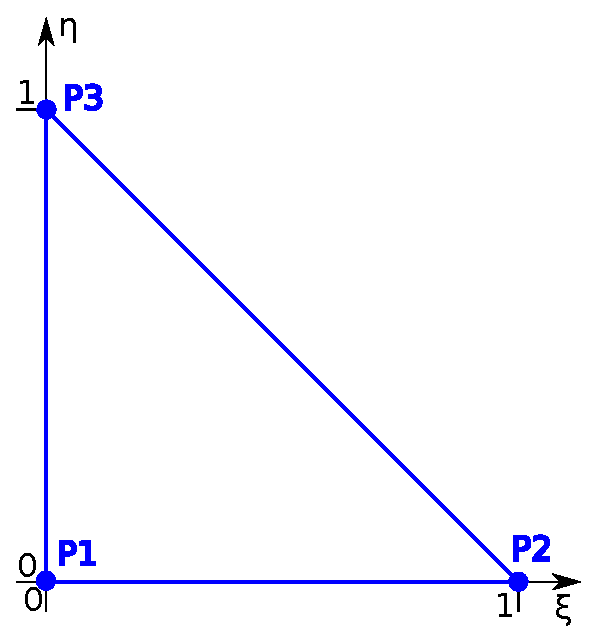
\includegraphics[scale=0.65]{pics/linear_element.eps}
	\end{center}
	\caption{Ansatz für lineares Element}
	\label{fig:linear_element}
\end{wrapfigure}

Die Koordinaten der drei Elementknoten lauten wie folgt:
\begin{align}
&P_1 = \coord{0}{0}, \quad P_2 = \coord{0}{1} \\
&P_3 = \coord{1}{0} \nonumber
\end{align}

Als Ansatz für die Potentialfunktion bzw. die globalen Koordinaten $x$ und $y$ wählt man folgenden Ansatz:
\begin{equation}
 \label{eq:linear_triangle_eq}
u(\xi, \eta) = c_0 + c_1 \xi + c_2 \eta
\end{equation}
Die drei Unbekannten $c_0$, $c_1$ und $c_2$ können durch Einsetzen der Koordinaten der Elementknoten ermittelt werden. 
\begin{align}
P_1:&\ u(0,0) = u_1 = c_0\\
P_2:&\ u(1,0) = u_2 = c_0 + c_1 \nonumber \\
P_3:&\ u(0,1) = u_3 = c_0 + c_2 \nonumber
\end{align}
 bzw. unter Verwendung der Matrixschreibweise:
 \begin{equation}
 \label{eq:linear_triangle_matrix_eq}
 \underbrace{
 \begin{bmatrix}
 1 & 0 & 0 \\
 1 & 1 & 0 \\
 1 & 0 & 1
 \end{bmatrix}}_{\mat{A}} \cdot 
\underbrace{
 \begin{Bmatrix}
 c_0 \\ c_1 \\ c_2
 \end{Bmatrix}}_{\vec{c}} = 
\underbrace{
 \begin{Bmatrix}
 u_1 \\ u_2 \\ u_3
 \end{Bmatrix}}_{\vec{u}}
 \end{equation}
 
 Die Lösung $\vec{c} = \mat{A}^{-1}\cdot\vec{u}$ lautet:
 \begin{equation}
\begin{Bmatrix}
c_0 \\ c_1 \\ c_2
\end{Bmatrix} = 
\begin{bmatrix}
1 & 0 & 0 \\
-1 & 1 & 0 \\
-1 & 0 & 1
\end{bmatrix}
 \cdot 
 \begin{Bmatrix}
 	u_1 \\ u_2 \\ u_3
 \end{Bmatrix}
\end{equation}
Oder ausgeschrieben:
\begin{align}
	c_0 &= u_1 \\
	c_1 &= u_2 - u_1 \nonumber\\
	c_2 &= u_3 - u_1 \nonumber
\end{align}

Setzt man dies wiederum in (\ref{eq:linear_triangle_eq}) ein, so erhält man:
\begin{equation}
u(\xi, \eta) = u_1 + (u_2 - u_1)\xi + (u_3 - u_1)\eta
\end{equation}
bzw. nach einfacher Umformung:
\begin{equation}
u(\xi, \eta) = \underbrace{(1 - \xi - \eta)}_{N_1} u_1 + \underbrace{(\xi)}_{N_2} u_2 + \underbrace{(\eta)}_{N_3} u_3
\end{equation}

Die Formfunktionen für das lineare finite Dreieckselement lauten also:
	\begin{align}
		N_1(\xi, \eta) &= 1 - \xi - \eta \\
		N_2(\xi, \eta) &= \xi \nonumber \\
		N_3(\xi, \eta) &= \eta \nonumber
	\end{align}
	
	
	
	
% =============================== Quadratische Elemente ======================================

\subsubsection{Quadratische Dreieckselemente}
Das quadratische isoparametrische finite Dreieckselement ist wie in Abbildung \ref{fig:quadratic_element} definiert.

Die Koordinaten der drei Elementknoten lauten wie folgt:
\begin{align}
&P_1 = \coord{0}{0}, \quad P_2 = \coord{\nicefrac{1}{2}}{0}\\
&P_3 = \coord{1}{0}, \quad P_4 = \coord{\nicefrac{1}{2}}{\nicefrac{1}{2}} \nonumber \\
&P_5 = \coord{0}{1}, \quad P_6 = \coord{0}{\nicefrac{1}{2}} \nonumber
\end{align}

\begin{wrapfigure}{r}{8cm}
	\begin{center}
		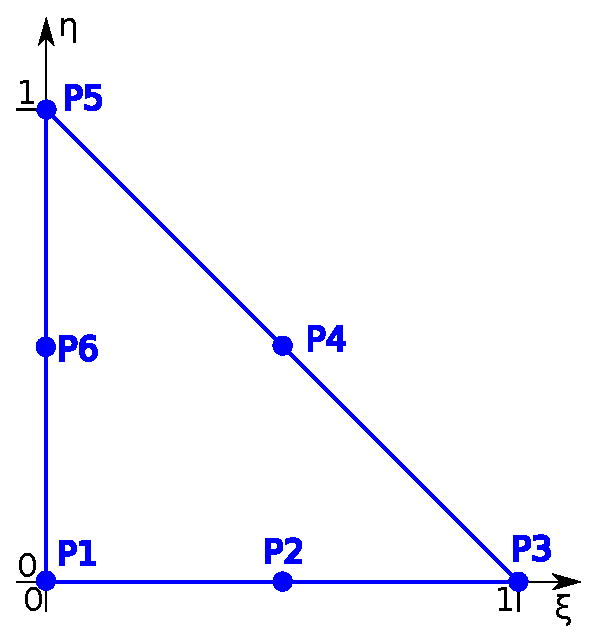
\includegraphics[scale=0.65]{pics/quadratic_element.eps}
	\end{center}
	\caption{Ansatz für quadratisches Element}
	\label{fig:quadratic_element}
\end{wrapfigure}

Der Ansatz der Potentialfunktion wird wie folgt gewählt:
\begin{equation}
\label{eq:quadratic_triangle_eq}
u(\xi, \eta) = c_0 + c_1 \xi + c_2 \eta + c_3 \xi \eta + c_4 \xi^2 + c_5 \eta^2
\end{equation}	
Nach dem Einsetzen der Knotenkoordinaten ergeben sich folgende Gleichungen zur Bestimmung der Unbekannten $c_j$:
\begin{align}
&u(0,0) = u_1 = c_0\\
&u(\nicefrac{1}{2}, 0) = u_2 = c_0 + \frac{1}{2} c_1 + \frac{1}{4} c_4 \nonumber \\
&u(1, 0) = u_3 = c_0 + c_1 + c_4 \nonumber \\
&u(\nicefrac{1}{2}, \nicefrac{1}{2}) = u_4 = c_0 + \frac{1}{2} c_1 + \frac{1}{2} c_2 + \frac{1}{4} c_3 + \frac{1}{4} c_4  \nonumber \\ 
&\quad \quad \quad \quad \quad \quad \quad \quad \ +\frac{1}{4} c_5\nonumber \\
&u(0, 1) = u_5 = c_0 + c_2 + c_5 \nonumber \\
&u(\nicefrac{1}{2}, 0) = u_6 = c_0 + \frac{1}{2} c_2 + \frac{1}{4} c_5 \nonumber
\end{align}		

Durch Anwendung des gleichen Prinzips wie in Abschnitt \ref{sec:linear_triangles} können nun die Formfunktionen $N_1 \text{...} N_6$ ermittelt werden. Diese finden sich in Anhang ... .




% =============================== Kubische Elemente ======================================

\subsubsection{Kubische Dreieckselemente}

Das kubische isoparametrische finite Dreieckselement ist wie in Abbildung \ref{fig:cubic_element} definiert.

\begin{wrapfigure}{r}{8cm}
	\vspace{-6cm}
	\begin{center}
		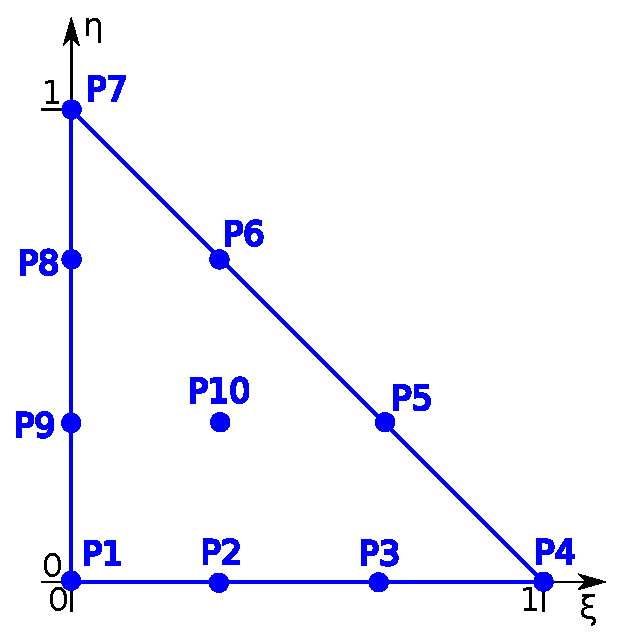
\includegraphics[scale=0.65]{pics/cubic_element.eps}
	\end{center}
	\caption{Ansatz für quadratisches Element}
	\label{fig:cubic_element}
\end{wrapfigure}

Die Koordinaten der drei Elementknoten lauten wie folgt:
\begin{align}
&P_1 = \coord{0}{0}, \quad P_2 = \coord{\nicefrac{1}{3}}{0}\\
&P_3 = \coord{\nicefrac{2}{3}}{0}, \quad P_4 = \coord{1}{0} \nonumber \\
&P_5 = \coord{\nicefrac{2}{3}}{\nicefrac{1}{3}}, \quad P_6 = \coord{\nicefrac{1}{3}}{\nicefrac{2}{3}} \nonumber\\
&P_7 = \coord{0}{1}, \quad P_8 = \coord{0}{\nicefrac{2}{3}} \nonumber \\
&P_9 = \coord{0}{\nicefrac{1}{3}}, \quad P_10 = \coord{\nicefrac{1}{3}}{\nicefrac{1}{3}} \nonumber\\
\end{align}

Der Ansatz der Potentialfunktion wird wie folgt gewählt:

\begin{equation}
\label{eq:cubic_triangle_eq}
u(\xi, \eta) = c_0 + c_1 \xi + c_2 \eta + c_3 \xi \eta + c_4 \xi^2 + c_5 \eta^2 + c_6 \xi^2 \eta + c_7 \xi \eta^2 + c_8 \xi^3 + c_9 \eta^3
\end{equation}	



Nach dem Einsetzen der Knotenkoordinaten ergeben sich folgende Gleichungen zur Bestimmung der Unbekannten $c_j$:
\begin{align}
u(0,0) = &u_1 = c_0\\
u(\nicefrac{1}{3}, 0) = &u_2 = c_0 + \frac{1}{3} c_1 + \frac{1}{9} c_4 +  \frac{1}{27} c_8\nonumber \\
u(\nicefrac{2}{3}, 0) = &u_3 = c_0 + \frac{2}{3} c_1 + \frac{4}{9} c_4 +  \frac{8}{27} c_8\nonumber \\
u(1,0) = &u_4 = c_0 + c_1 + c_4 + c_8\nonumber\\
u(\nicefrac{2}{3}, \nicefrac{1}{3}) = &u_5 = c_0 + \frac{2}{3} c_1 +  \frac{1}{3} c_2 + \frac{2}{9} c_3 +  \frac{4}{9} c_4 + \frac{1}{9} c_5 + \frac{4}{27} c_6 + \frac{2}{27} c_7 + \frac{8}{27} c_8 + \frac{1}{27} c_9\nonumber\\
u(\nicefrac{1}{2}, 0) = &u_6 = c_0 + \frac{1}{3} c_1 +  \frac{2}{3} c_2 + \frac{2}{9} c_3 +  \frac{1}{9} c_4 + \frac{4}{9} c_5 + \frac{2}{27} c_6 + \frac{4}{27} c_7 + \frac{1}{27} c_8 + \frac{8}{27} c_9\nonumber\\
u(0,1) = &u_7 = c_0 + c_2 + c_5 + c_9\nonumber\\
u(0, \nicefrac{2}{3}) = &u_8 = c_0 + \frac{2}{3} c_2 + \frac{4}{9} c_5 +  \frac{8}{27} c_9\nonumber \\
u(0, \nicefrac{1}{3}) = &u_9 = c_0 + \frac{1}{3} c_2 + \frac{1}{9} c_5 +  \frac{1}{27} c_9\nonumber \\
u(\nicefrac{1}{3}, \nicefrac{1}{3}) = &u_{10} = c_0 + \frac{1}{3} c_1 +  \frac{1}{3} c_2 + \frac{1}{9} c_3 +  \frac{1}{9} c_4 + \frac{1}{9} c_5 + \frac{1}{27} c_6 + \frac{1}{27} c_7 + \frac{1}{27} c_8 + \frac{1}{27} c_9\nonumber
\end{align}	
	

Durch Anwendung des gleichen Prinzips wie in Abschnitt \ref{sec:linear_triangles} können nun die Formfunktionen $N_1 \text{...} N_10$ ermittelt werden. Diese finden sich in Anhang ... .
\subsection{Problemtypen}
In diesem Kapitel werden die in der Software implementierten Problemtypen beschrieben. In beiden Fällen handelt es sich um zweidimensionale, ebene Probleme. Resultat dieses Abschnitts werden analytische Berechnungsvorschriften für die einzelnen Elementgleichungssysteme sein.\newline
Die Berechnungen aus diesem Abschnitt stammen, sofern nicht anders angegeben, aus \cite{SMS_VO_skript} Kapitel 7 und 8. Für ausführliche Herleitungen, auf welche in diesem Fall bewusst verzichtet wird, sei auf das oben genannte Werk verwiesen.\newline

Wie aus Abschnitt \ref{sec:fem_theory} bekannt, ist das Randwertproblem zuerst als Operatorgleichung mit entsprechenden Randwertbedingungen zu formulieren. Die Operatorgleichung kann nun entweder direkt im Galerkinschen Verfahren oder über Umweg eines äquivalenten Funktionals im Ritzschen Verfahren verwendet werden. Dabei wird für die gesuchte Funktion $u$ in jedem Teilgebiet (finites Element) ein entsprechender Approximations-Ansatz wie in Abschnitt \ref{sec:finite_elements_and_shape_functions} ermittelt, eingesetzt. Das Ergebnis sind 'lokale' lineare Gleichungssysteme (für jedes Element eines), welche zu einem großen, 'globalen' Gleichungssystem assembliert werden müssen. Auf die Assemblierung wird dabei genauer in Abschnitt \ref{sec:assembling} eingegangen.\newline

Ausgangspunkt für Probleme aus der Elektrotechnik sind im Allgemeinen die Maxwell-Gleichungen:
\begin{align}
	\mathit{rot}\vec{E} = -\parDiff{\vec{B}}{t} \label{eq:maxwell_1} \\
	\mathit{rot}\vec{H} = \vec{J} + \parDiff{\vec{D}}{t} \label{eq:maxwell_2}\\
	\mathit{div}\vec{B} = 0 \label{eq:maxwell_3}\\
	\mathit{div}\vec{D} = \rho \label{eq:maxwell_4}
\end{align}
mit den Materialzusammenhängen
\begin{align}
\vec{D} = [\epsilon]\vec{E} \label{eq:material_1}\\
\vec{B} = [\mu]\vec{H} \label{eq:material_2}
\end{align}
mit $[\epsilon]$ und $[\mu]$ als ortsabhängigen Materialtensoren.

\subsubsection{Elektrostatische Probleme}
\label{sec:electrostatic_problems}
Für den elektrostatischen Fall ist $\vec{J},\ \vec{H}$, sowie sämtliche zeitlichen Änderungen $\equiv 0$ wodurch sich $\vec{B}$ sowie die rechte Seite von (\ref{eq:maxwell_1}) zu $\equiv 0$ ergeben.\newline
Ein elektrostatisches Problem wird somit durch die folgenden Gleichungen beschrieben:
\begin{align}
\mathit{rot}\vec{E} &= 0 \label{eq:wirbelfreiheit_E}\\
\mathit{div}\vec{D} &= \rho \label{eq:sources_D}
\end{align}\newline

Aufgrund der Wirbelfreiheit des elektrischen Feldes aus (\ref{eq:wirbelfreiheit_E}) kann nun folgender Ansatz für die elektrische Feldstärke $\vec{E}$ verwendet werden:
\begin{equation}
\label{eq:dgl_E}
\vec{E} = -\mathit{grad}V
\end{equation}
mit $V$ als sogenanntem \textit{Skalapotential}.\newline

Setzt man (\ref{eq:dgl_E}) nun unter Verwendung von (\ref{eq:material_1}) in (\ref{eq:sources_D}) ein, so erhält man die partielle Differentialgleichung für $V$ als:
\begin{equation}
\mathit{div}[\epsilon]\mathit{grad}V = -\rho
\end{equation}
Hierbei entspricht $\mathit{div}[\epsilon]\mathit{grad}$ dem Differentialoperator $L$ aus (\ref{eq:operatorgleichung}), das Potential $V$ der gesuchten Funktion $u$ und $-\rho$ der gegebenen Funktion $f$.\newline

Die Randbedingungen für ein solches Problem sind gegeben als
\begin{equation}
\label{eq:e-static_dirichlet_condition}
	V = \overline{V}
\end{equation}
am dirichletschen Rand $\Gamma_D$ und 
\begin{equation}
\label{eq:e-static_neumann_condition}
\vec{n}\cdot\mathit{grad}V = \sigma 
\end{equation}
am neumannschen Rand $\Gamma_N$, mit $\vec{n}$ als Flächennormale und $\sigma$ als gegebener Flächenladungsdichte.\newline

Unter Verwendung des Ritzschen \textit{oder} Galerkinschen Verfahrens erhält man nun Formeln zur Berechnung der Elementgleichungssysteme, wobei beide Verfahren dieselben (!) Formeln liefern. Löst man (\ref{eq:first_variation}) oder (\ref{eq:weighted_residuum}) mit den entsprechenden Ansätzen, so ergibt sich für jedes Element ein quadratisches lineares \textit{Elementgleichungssystem} $\begin{bmatrix}k_{ij}\end{bmatrix} \cdot \begin{Bmatrix}V_j\end{Bmatrix} = \begin{Bmatrix}r_j\end{Bmatrix}$ der Dimension $N\times N$ mit $N$ als Anzahl der Elementknoten.
\begin{equation}
\label{eq:k_ij_e_static}
k_{ij} = \int\displaylimits_{x} \int\displaylimits_{y} \left(\epsilon_x \parDiff{N_i}{x}\parDiff{N_j}{x} +  \epsilon_y\parDiff{N_i}{y}\parDiff{N_j}{y}\right)dx dy
\end{equation}


\begin{equation}
\label{eq:right_side_e_static}
	r_j = \int\displaylimits_{x} \int\displaylimits_{y} N_i \rho dx dy + \int\displaylimits_{\Gamma_N} N_i\sigma d\Gamma
\end{equation}

\textbf{Anmerkung:} Um auf die oben gezeigte Form für $k_ij$ zu kommen ist es notwendig den Permettivitätstensor $[\epsilon]$ auf die Hauptachsenform zu transformieren:
\begin{equation*}
	[\epsilon] = \begin{bmatrix}
	\epsilon_x & 0 \\
	0 & \epsilon_y
	\end{bmatrix}
\end{equation*}

Man beachte dass für Formfunktionen von isoparametrischen finite Elementen $N_i = N_i(\xi, \eta)$ gilt, wodurch alle Integrale in den Variablen $\xi$ und $\eta$ durchgeführt werden müssen. Die entsprechende Substitution sowie die Realisierung der Integrale werden in Abschnitt \ref{sec:equation_system_calculation} genauer behandelt. 


\subsubsection{Stationäre Strömungsfeldprobleme}
\label{sec:stat_current_problems}
Stationäre Strömungsfeldprobleme lassen sich über das Gesetz der Ladungserhaltung definieren:
\begin{equation}
	\mathit{div}\vec{J} = 0
\end{equation}
 Es muss außerdem das Ohmsche Gesetz in seiner differentiellen Form gelten:
 \begin{equation}
 	\vec{J} = [\gamma] \vec{E}
 \end{equation}
 mit $[\gamma]$ als ortsabhängigem Tensor der spezifischen Leitfähigkeit.\newline
 
 Stationäre Strömungsfeldprobleme können somit analog zu elektrostatischen Problemen mittels folgender Differentialgleichung ermittelt werden:
 \begin{equation}
\mathit{div}[\gamma]\mathit{grad}V = 0
 \end{equation}
 Als Randbedingungen ergeben sich:
 \begin{equation}
 \label{eq:current_dirichlet_condition}
 V = \overline{V}
 \end{equation}
 am dirichletschen Rand $\Gamma_D$ und 
 \begin{equation}
 \label{eq:current_neumann_condition}
 \vec{n}\cdot\mathit{grad}V = J_e
 \end{equation}
 am neumannschen Rand $\Gamma_N$, wobei $J_e$ die eingeprägte Flächenstromdichte am Rand darstellt.\newline
 
 Man erkennt die starken Äquivalenzen zwischen stationären Strömungsfeldproblemen und elektrostatischen Problemen. Das Elementgleichungssystem ergibt sich somit für diese Probleme als
 
\begin{equation}
\label{eq:k_ij_stat_current}
k_{ij} = \int\displaylimits_{x} \int\displaylimits_{y} \left(\gamma_x \parDiff{N_i}{x}\parDiff{N_j}{x} +  \gamma_y\parDiff{N_i}{y}\parDiff{N_j}{y}\right)dx dy
\end{equation}

\begin{equation}
\label{eq:right_side_stat_current}
r_j = \int\displaylimits_{x} \int\displaylimits_{y} N_i J_e dx dy
\end{equation}








\section{Implementierung}
Dieses Kapitel beschäftigt sich mit diversen Details der Implementierung des finite Elemente Algorithmus in der Software. Es wird beschrieben wie mittels der Software Gmsh die Problemgeometrie erstellt, sowie ein finite Elemente Gitter generiert und exportiert wird. Anschließend erfolgt ein kurzer Umriss des Imports und Verarbeitung des Gitters zur Verwendung im eigentlichen Lösungsalgorithmus auf den detaillierter am Ende dieses Kapitels eingegangen wird.

\subsection{Formulierung der finiten Elemente (gesamt: 3 Seiten)}
\subsubsection{3-Punkte linear (1 Seite)}
\subsubsection{6-Punkte quadratisch (1 Seite)}
\subsubsection{10-Punkte kubisch (1 Seite)}

\subsection{Erstellung der Geometrie und Generierung des Gitters mit Gmsh (gesamt: 3 Seiten)}
\subsubsection{Erstellen der Geometrie (2 Seiten)}
\subsubsection{Generierung und Export des FEM-Gitters (1 Seiten)}

\subsection{Import und Verarbeitung des FEM-Gitters (gesamt: 4 Seiten)}
\subsubsection{Import (1 Seiten)}
\subsubsection{Ermitteln der Knoten am dirichletschen Rand (1 Seiten)}
\subsubsection{Ermitteln der Element-Seiten am neumannschen Rand (2 Seite)}

\subsection{Berechnung der Elementgleichungssysteme (gesamt: 3 Seiten)}
\label{sec:equation_system_calculation}
\subsubsection{Berechnung der Element-Matrix (2 Seite)}
\subsubsection{Berechnung des Rechtsseiten-Vektors (1 Seite)}

\subsection{Assemblierung und Lösung des globalen Gleichungssystems (gesamt: 1 Seite)}
\label{sec:assembling}

\section{Simulationen}
\subsection{Simulation 1 (2 Seiten)}
\subsection{Simulation 2 (2 Seiten)}
\subsection{Simulation 3 (2 Seiten)}


\newpage
\addcontentsline{toc}{section}{Literatur}
\bibliography{literatur}

\end{document}